\chapter{Применение описанных подходов на практике}

В настоящей главе описывается эксперимент, в котором применялся
подход, описанный в главе~\ref{ch:problem_solving}, на
конкретной задаче определения демографических характеристик
пользователей с использованием конкретного набора данных.

В разделе~\ref{sec:dataset} произведён обзор набора данных,
который использовался в эксперименте, а также описана
конкретная задача, которая решалась.

В разделе~\ref{sec:algorithms_config} описаны применяемые
алгоритмы, а также их конфигурация.

В разделе~\ref{sec:result_quality} описан способ измерения
качества результата.

Наконец, в разделе~\ref{sec:results} приведены результаты,
полученные в результате проведения эксперимента.

\section{Описание набора данных}
\label{sec:dataset}

Для подтверждения состоятельности описанного подхода к решению задачи
профилирования пользователей на основе анализа их музыкальных
интересов был проведён эксперемент. Решалась задача определения
демографических характеристик (пола и возраста) пользователей сайта 
Last.fm с использованием набора данных, который использовался в
работе~\cite{wu2014gender}.

Авторы упомянутой работы загружали данные с сайта Last.fm. Всего набор
данных содержит 96807 пользовтель. Для каждого пользователя была
получена информация о его музыкальных интересах при помощи метода
публичного API сайта \textit{User.getTopTracks}, который возвращает
50 наиболее прослушиваемых музыкальных композиций заданным пользователем. 
Музыкальные композиции отсортированы в порядке убывания числа прослушиваний.
При этом данные содержат только имена исполнителей, извлечённые из этого списка.
То есть данные имеют такой вид, который был описан в 
разделе~\ref{sec:problem_formulation}. 

Кроме того, при помощи метода API сайта \textit{User.getInfo}
была получена информация о поле и возрасте для каждого пользователя.

Каждый пользователь в наборе описан по меньшей мере 40
музыкальными композициями. У каждого пользователя указан пол и возраст.
Набор данных содержит 133938 уникальных музыкальных исполнителей.

Стоит также отметить некоторые особенности выборки пользователей.
Во-первых, мужчин в ней содержится больше, чем женщин. Распределение
пола в выборке проиллюстрировано на рисунке~\ref{fig:gender_pie}.
Во-вторых, распределение возраста в выборке не является равномерным,
и оно смещено в сторону молодого поколения. Медиана распределения
возраста в выборке равна 31, а средний возраст равен 29,05.
Распределение возраста в выборке пользователей изображено на
рисунке~\ref{fig:age_histogram}.

Используя данные о музыкальных исполнителях пользователей,
решалось две задачи~--- задача определения пола и задача
определения возраста. Первая задача решалась как задача
бинарной классификации, а вторая~--- как задача восстановления
регрессии.

\begin{figure}[!h]
\caption{Распределение пола в выборке пользователей}
\label{fig:gender_pie}
\centering
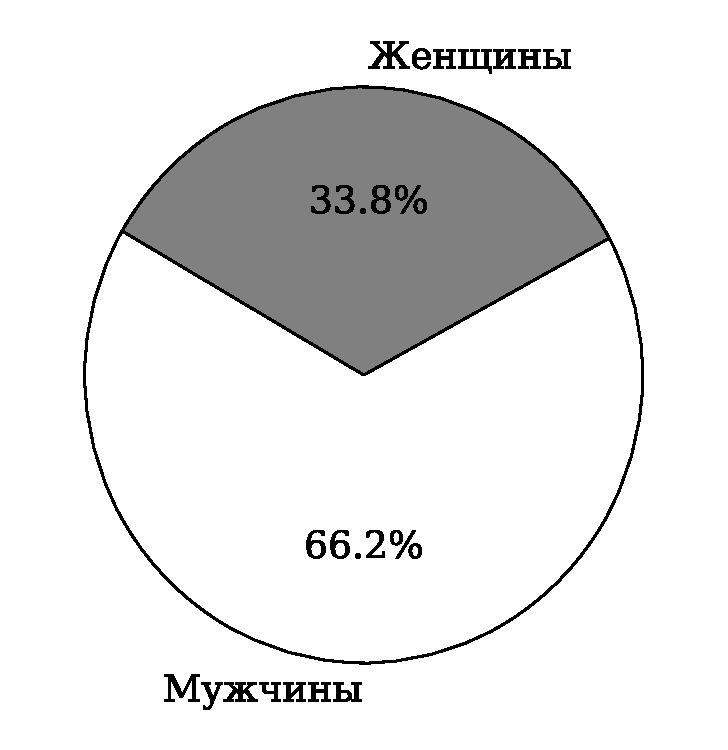
\includegraphics[scale=0.65]{figs/gender-pie.pdf}
\end{figure}

\begin{figure}[!h]
\caption{Распределение возраста в выборке пользователей}
\label{fig:age_histogram}
\centering
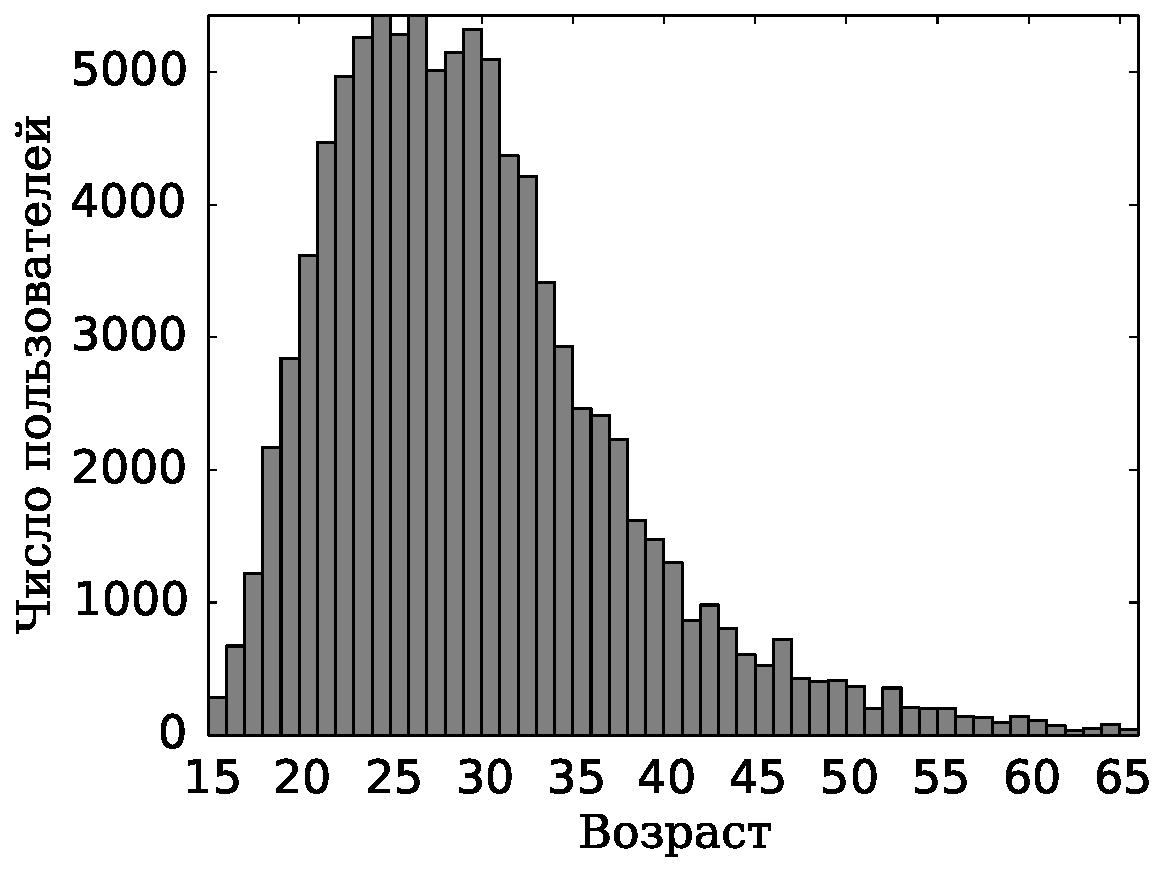
\includegraphics[scale=0.60]{figs/age-histogram.pdf}
\end{figure}

\section{Используемые алгоритмы и их конфигурация}
\label{sec:algorithms_config}

В данном разделе описаны используемые алгоритмы латентного
семантического анализа, техники word embedding, а также методов
классификации и восстановления регрессии. Кроме всего, приведены
конфигурации алгоритмов.

\subsection{Алгоритмы латентного семантического анализа}

В качестве алгоритмов латентного семантического анализа
в эксперименте использовались алгоритмы PLSA (реализация из библиотеки
\textit{BigARTM}~\cite{bigartm}), LDA (реализция из библиотеки
\textit{gensim}~\cite{gensim}) и LSI (реализация из библиотеки
\textit{gensim}).

Стоит отметить, что при использовании алгоритмов
\textit{PLSA} и \textit{LDA} результаты получались похожими 
на случайные, поэтому детальные эксперементы с их 
использованием не проводились. 

Возможно, такое поведение объясняется тем фактом, 
что их использование основано на гипотезе о существовании 
латентных жанров исполнителей, но часто не существует единогласного 
мнения о жанрах, которые исполняет тот или иной музыкальный исполнитель.
Поэтому можно считать, что данная гипотеза не выполняется.

Также имеет место предположение о том, что в большинстве случаев
люди предпочитают слушать музыку различных жанров, поэтому жанры
являются неинформативными признаками.

Напротив, использование алгоритма \textit{LSI} позволяет получить хорошие
результаты. Именно он и использовался в детальных экспериментах.

В качестве числа тематик в алгоритме \textit{LSI} использовалось
два значения~--- 200 тематик и 20 тематик. 
Для остальных параметров алгоритма использовались значения по умолчанию.

\subsection{Алгоритмы векторного представления слов}

В качестве алгоритма, реализующего модель векторного представления
слов использовался алгоритм Word2Vec, именно его реализация из
библиотеки \textit{gensim}.  

В качестве размерности векторов использовалось два значения~--- 200
и 20 (параметр \textit{size}).

Шириной контекста было выбрано значение 50 (параметр \textit{window}),
что означает использование в качестве контекста всех исполнителей для
любого из пользователей.

Для остальных параметров алгоритма Word2Vec использовались значения
по умолчанию.

\subsection{Алгоритмы классификации и восстановления регрессии}

В качестве алгоритма классификации или восстановления регресии
использовался \textit{метод опорных векторов (Support Vector Machine,
SVM)}~\cite{cortes1995support} с ядром 
\textit{radial basis function (RBF)}. Использовалась реализация
метода опорных векторов из программной библиотеки 
\textit{scikit-learn}~\cite{sklearn}, а именно алгоритмы
\textit{SVC} и \textit{SVR} для задач классификации и регрессии
соответственно.

Параметры метода опорных векторов \textit{C} и \textit{gamma},
выбор которых во многих задачах сильно влияет на результат,
настраивались на обучающей выборке (подробнее о разбиении
на обучающую и контрольную выборку см.
раздел~\ref{sec:result_quality}) методом \textit{GridSearchCV},
который реализован в библиотеке \textit{scikit-learn}. Множества
параметров \textit{C} и \textit{gamma} были выбраны следующие:
\[
    C \in \{0; 1; 0.5; 1; 3\},\quad
    \mathrm{gamma} \in \{0.001; 0.01; 0.1; 1; 8; 16; 32; 64\}.
\]

Метод \textit{GridSearchCV} использует \textit{кросс-валидацию}
с разбиением на $k$ частей (\textit{k-fold cross validation}).
Было выбрано число разбиений равное трём.

Для задачи определения пола параметры подбирались таким
образом, чтобы максимизировать точность классификации (подробнее
см. раздел~\ref{sec:result_quality}).

Для задачи определения возраста параметры подбирались так, чтобы
минимизировать среднюю абсолютную ошибку (подробнее см.
раздел~\ref{sec:result_quality}).

Перед использованием алгоритма классификации или регрессии
вектора пользователей были нормализованы по $L_2$ норме
(при использовании латентного семантического анализа) или
стандартизованы (при использовании подхода на основе
векторного представления слов).

\section{Способ измерения качества результата}
\label{sec:result_quality}

Разбиение выборки пользователь на обучающую и контрольную
было произведено случайным образом, но так, чтобы распределение
пола в каждой из выборок было одинаковым.

Обучающая выборка содержит 48404 пользователей, а контрольная~---
48403 пользователей.

Стоит отдельно отметить, что разбиение выборки пользователей на
обучающую и контрольную было произведено \textit{в точности таким
же образом}, как это было сделано в работе~\cite{wu2014gender}.

Обучение происходило на обучающей выборке, а качество классификации
или восстановления регрессии измерялось на контрольной выборке
с использованием метрик. Опишем этим метрики. 


Пусть имеется матрица <<пользователь-признак>>
$X \in \mathbb{R}^{n \times m}$. Будем обозначать вектор,
описывающий пользователя $i$ как $\bm{x}_i$ (строка матрицы $X$).
Множество этих векторов будем обозначать как $\mathcal{X}$.
Также пусть для каждого пользователя с номером $i$ имеются метки,
обозначающие пол пользователя, $g_i \in G$ и метки, обозначающие
возраст~--- $a_i \in A$. Тогда метрика для определения качества
классификации (называемая \textit{точностью}) будет иметь следующий вид:
\[
    \mathrm{ACC} = 
    100\% \cdot \frac{1}{n} \cdot 
    \sum_{i=1}^{n}[g_i = \mathcal{C}(\bm{x}_i)],
    \quad \mathcal{C} \colon \mathcal{X} \mapsto G,
\]
где $\mathcal{C}$~--- алгоритм классификации. А метрика для оценки
качества восстановления регресии (называемая \textit{средней
абсолютной ошибкой}) вычисляется по формуле:
\[
    \mathrm{MAE} =
    \frac{1}{n} \cdot \sum_{i=1}^{n} 
    \left|a_i - \mathcal{R}(\bm{x}_i)\right|,
    \quad \mathcal{R} \colon \mathcal{X} \mapsto A,
\]
где $\mathcal{R}$~--- алгоритм восстановления регрессии.

Большое значение точности характеризует высокое качество классификации.
Малое значение средней абсолютной ошибки характеризует высокое качество
восстановления регрессионной зависимости.

Ввиду того, что распределение пола в выборке пользователей
является неравномерным, в результатах также будут приведены
\textit{матрицы ошибок (error matrix, confusion matrix)
}~\cite{stehman1997selecting} для задач классификации.
Данные матрицы показывают число верно и неверно классифицированных
объектов для каждого из классов.

\section{Результаты}
\label{sec:results}

В данном разделе приведены результаты, полученные в результате
эксперимена с применением подхода, описанного в 
главе~\ref{ch:problem_solving}.

В таблице~\ref{tab:bow_lsa}
приведены результаты с использованием подхода <<bag of words>>
для вычисления матрицы <<исполнитель-пользователь>> и латентного
семантического анализа для построения матрицы <<пользователь-признак>>.
Для вычисления элементов матрицы <<исполнитель-пользователь>> использовалась
обобщённая формула TF-IDF (см. формулу~\ref{eq:general_tfidf}) с
использованием различных функций $l$ и $g$, а также формула
log-entropy (см. формулу~\ref{eq:log_entropy}). Как видно,
добиться наилучших результатов позволяет простейший подход,
при котором элемент $d_{ij}$ матрицы <<исполнитель-пользователь>>
равен единице, если исполнитель $i$ встречается у пользователя $j$,
и нулю~--- иначе. Для модели, позволяющей достигнуть лучших
результатов в задаче определения пола,
на рисунке~\ref{fig:bow_lsa_conf} приведены матрицы ошибок.

\begin{table}[!h]
    \caption{Результаты эксперимента с применением подходов
            <<bag of words>> и латентного семантического анализа}
    \label{tab:bow_lsa}
\centering
\begin{tabular}{|c|c|c|c|c|}\hline
    \textbf{Формула} & \boldmath$l(x)$ & \boldmath$g(x)$ & \textbf{Определение пола} & \textbf{Определение возраста} \\\hline
    \multicolumn{5}{|c|}{\textbf{20 признаков}} \\\hline
    TF-IDF & $1$ & $1$ & \textbf{73,33\%} & \textbf{4,72} \\\hline
    TF-IDF & $\log{x}$ & $1$ & 72,83\% & 4,80 \\\hline
    TF-IDF & $\log{x}$ & $\log{x}$ & 70,56\% & 4,91 \\\hline
    TF-IDF & $\log{x}$ & $\sqrt{x}$ & 67,08\% & 5,49 \\\hline
    TF-IDF & $\sqrt{x}$ & $1$ & 72,80\% & 4,79 \\\hline
    TF-IDF & $\sqrt{x}$ & $\log{x}$ & 70,61\% & 4,91 \\\hline
    TF-IDF & $\sqrt{x}$ & $\sqrt{x}$ & 67,07\% & 5,48 \\\hline
    TF-IDF & $x$ & $1$ & 70,74\% & 5,02 \\\hline
    TF-IDF & $x$ & $\log{x}$ & 69,38\% & 5,12 \\\hline
    TF-IDF & $x$ & $\sqrt{x}$ & 67,44\% & 5,45 \\\hline
    log-entropy & --- & --- & 71,15\% & 4,90 \\\hline
    \multicolumn{5}{|c|}{\textbf{200 признаков}} \\\hline
    TF-IDF & $1$ & $1$ & \textbf{82,46\%} & \textbf{3,54} \\\hline
    TF-IDF & $\log{x}$ & $1$ & 81,59\% & 3,64 \\\hline
    TF-IDF & $\log{x}$ & $\log{x}$ & 81,67\% & 3,58 \\\hline
    TF-IDF & $\log{x}$ & $\sqrt{x}$ & 80,08\% & 5,49 \\\hline
    TF-IDF & $\sqrt{x}$ & $1$ & 72,80\% & 4,79 \\\hline
    TF-IDF & $\sqrt{x}$ & $\log{x}$ & 70,61\% & 4,91 \\\hline
    TF-IDF & $\sqrt{x}$ & $\sqrt{x}$ & 67,07\% & 5,48 \\\hline
    TF-IDF & $x$ & $1$ & 70,74\% & 5,02 \\\hline
    TF-IDF & $x$ & $\log{x}$ & 69,38\% & 5,12 \\\hline
    TF-IDF & $x$ & $\sqrt{x}$ & 67,44\% & 5,45 \\\hline
    log-entropy & --- & --- & 81,46\% & 3,59 \\\hline
\end{tabular}
\end{table}

\begin{figure}[!h]
\caption{Матрицы ошибок для задачи определения пола с
         применением подходов <<bag of words>> и
         латентного семантического анализа}
\label{fig:bow_lsa_conf}
\centering
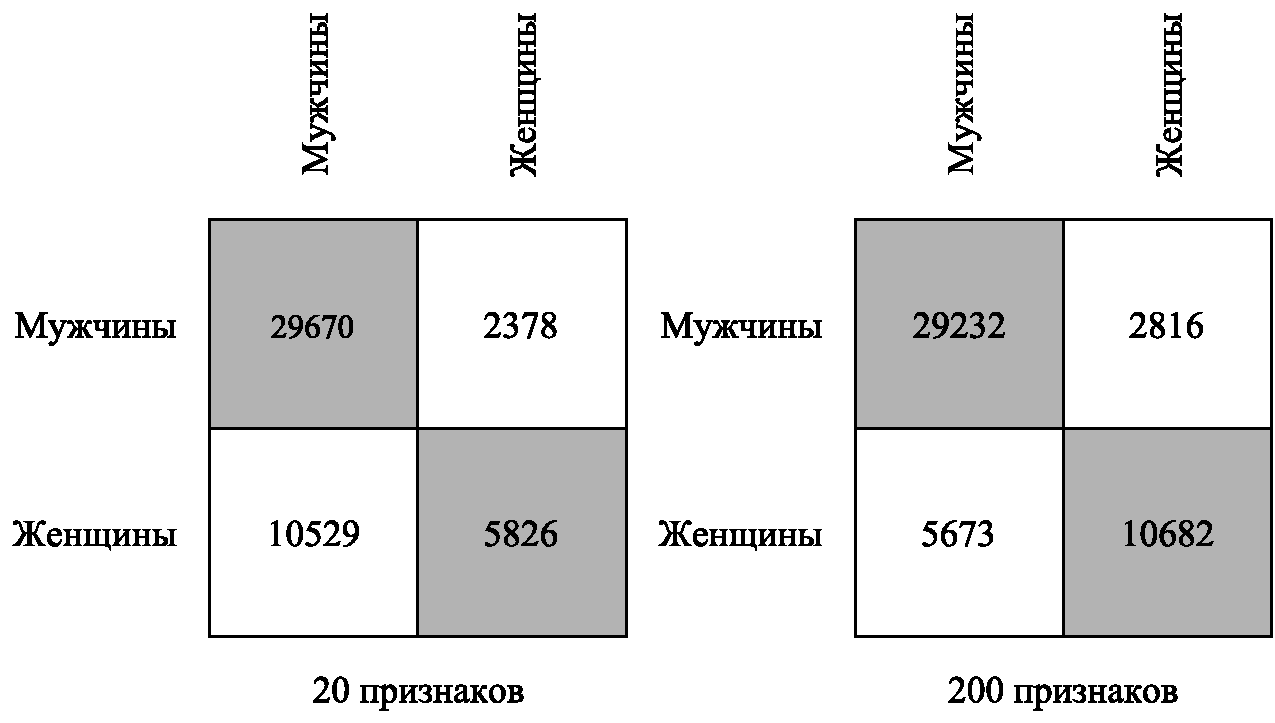
\includegraphics[scale=0.8]{figs/bow-lsa-confusion.pdf}
\end{figure}

В таблице~\ref{tab:order_lsa} приведены результаты эксперемента
с применением подхода вычисления матрицы <<исполнитель-пользователь>>
на основе порядка следования исполнителей (см. формулу~\ref{eq:order_dij})
при выборе различных функций $f$ и латентного семантического анализа.
Как видно, учёт подрядка следования исполнителей только ухудшает результат.
На рисунке~\ref{fig:order_lsa_conf} приведены матрицы ошибок для 
модели, позволяющей достигнуть лучших результатов в задаче определения
пола.

\begin{table}[!h]
    \caption{Результаты эксперимента с применением подходов
             вычисления матрицы <<исполнитель-пользователь>>
             на основе порядка следования исполнителей 
             и латентного семантического анализа}
    \label{tab:order_lsa}
\centering
\begin{tabular}{|c|c|c|}\hline
    \boldmath$f(a)$ & \textbf{Определение пола} & \textbf{Определение возраста} \\\hline
    \multicolumn{3}{|c|}{\textbf{20 признаков}} \\\hline
    $\frac{1}{\log(a + 1)}$ & \textbf{71,68\%} & \textbf{4,83} \\\hline
    $\frac{1}{\sqrt{a}}$ & 71,56\% & 4,90 \\\hline
    $\frac{1}{a^2}$ & 71,17\% & 4,97 \\\hline
    $\frac{1}{a}$ & 71,19\% & 4,93 \\\hline
    $51 - a$ & 71,38\% & 4,87 \\\hline
    $\log{51} - \log{a}$ & 71,02\% & 4,93 \\\hline
    $\sqrt{51} - \sqrt{a}$ & 70,96\% & 4,90 \\\hline
    \multicolumn{3}{|c|}{\textbf{200 признаков}} \\\hline
    $\frac{1}{\log(a + 1)}$ & \textbf{79,65\%} & \textbf{3,93} \\\hline
    $\frac{1}{\sqrt{a}}$ & 79,39\% & 3,97 \\\hline
    $\frac{1}{a^2}$ & 77,51\% & 4,06 \\\hline
    $\frac{1}{a}$ & 77,67\% & 4,13 \\\hline
    $51 - a$ & 79,01\% & 3,98 \\\hline
    $\log{51} - \log{a}$ & 78,73\% & 4,04 \\\hline
    $\sqrt{51} - \sqrt{a}$ & 79,02\% & 4,01 \\\hline
\end{tabular}
\end{table}

\begin{figure}[!h]
\caption{Матрицы ошибок для задачи определения пола с
         применением подходов вычисления матрицы 
         <<исполнитель-пользователь>> на основе порядка следования
         исполнителей и латентного семантического анализа}
\label{fig:order_lsa_conf}
\centering
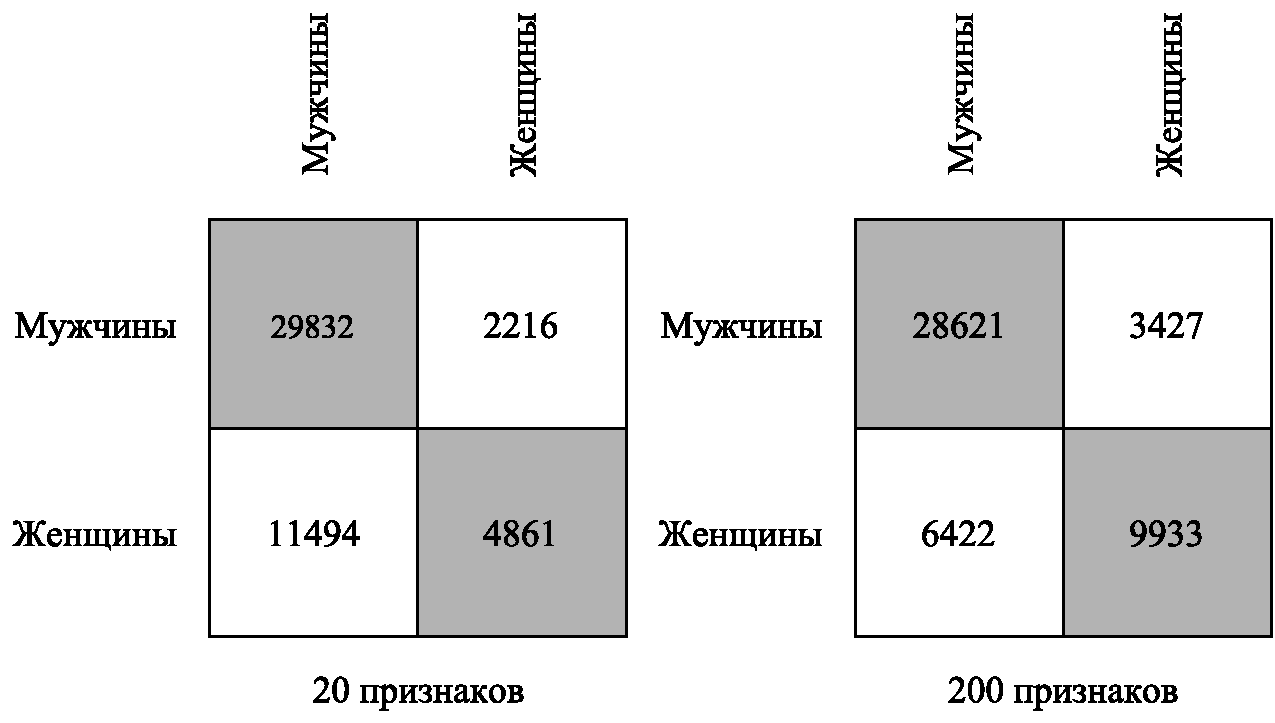
\includegraphics[scale=0.8]{figs/order-lsa-confusion.pdf}
\end{figure}

В таблице~\ref{tab:bow_we} приведены результаты эксперимента
с применением подхода <<bag of words>> и метода word embedding.
Для модели, позволяющей получить лучшие результаты в задаче
определения пола пользователей на рисунке~\ref{fig:bow_we_conf}
приведены матрицы ошибок.

\begin{table}[!h]
    \caption{Результаты эксперимента с применением подходов
            <<bag of words>> и word embedding}
    \label{tab:bow_we}
\centering
\begin{tabular}{|c|c|c|c|c|}\hline
    \textbf{Формула} & \boldmath$l(x)$ & \boldmath$g(x)$ & \textbf{Определение пола} & \textbf{Определение возраста} \\\hline
    \multicolumn{5}{|c|}{\textbf{20 признаков}} \\\hline
    TF-IDF & $1$ & $1$ & 79,59\% & 3,14 \\\hline
    TF-IDF & $\log{x}$ & $1$ & 79,32\% & 3,15 \\\hline
    TF-IDF & $\log{x}$ & $\log{x}$ & 78,06\% & 3,43 \\\hline
    TF-IDF & $\log{x}$ & $\sqrt{x}$ & 78,04\% & 3,43 \\\hline
    TF-IDF & $\sqrt{x}$ & $1$ & 78,33\% & 3,34 \\\hline
    TF-IDF & $\sqrt{x}$ & $\log{x}$ & 78,05\% & 3,43 \\\hline
    TF-IDF & $\sqrt{x}$ & $\sqrt{x}$ & 78,01\% & 3,43 \\\hline
    TF-IDF & $x$ & $1$ & 78,12\% & 3,40 \\\hline
    TF-IDF & $x$ & $\log{x}$ & 78,00\% & 3,43 \\\hline
    TF-IDF & $x$ & $\sqrt{x}$ & 78,00\% & 3,43 \\\hline
    log-entropy & --- & --- & \textbf{81,91\%} & \textbf{2,84} \\\hline
    \multicolumn{5}{|c|}{\textbf{200 признаков}} \\\hline
    TF-IDF & $1$ & $1$ & 78,98\% & 3,24 \\\hline
    TF-IDF & $\log{x}$ & $1$ & 78,26\% & 3,20 \\\hline
    TF-IDF & $\log{x}$ & $\log{x}$ & 78,05\% & 3,42 \\\hline
    TF-IDF & $\log{x}$ & $\sqrt{x}$ & 78,01\% & 3.43 \\\hline
    TF-IDF & $\sqrt{x}$ & $1$ & 78,21\% & 3,38 \\\hline
    TF-IDF & $\sqrt{x}$ & $\log{x}$ & 78,03\% & 3,43 \\\hline
    TF-IDF & $\sqrt{x}$ & $\sqrt{x}$ & 78,01\% & 3,43 \\\hline
    TF-IDF & $x$ & $1$ & 78,12\% & 3,41 \\\hline
    TF-IDF & $x$ & $\log{x}$ & 78,01\% & 3,43 \\\hline
    TF-IDF & $x$ & $\sqrt{x}$ & 78,00\% & 3,43 \\\hline
    log-entropy & --- & --- & \textbf{83,86\%} & \textbf{2,65} \\\hline
\end{tabular}
\end{table}

\begin{figure}[!h]
\caption{Матрицы ошибок для задачи определения пола с
         применением подходов <<bag of words>> и
         word embedding}
\label{fig:bow_we_conf}
\centering
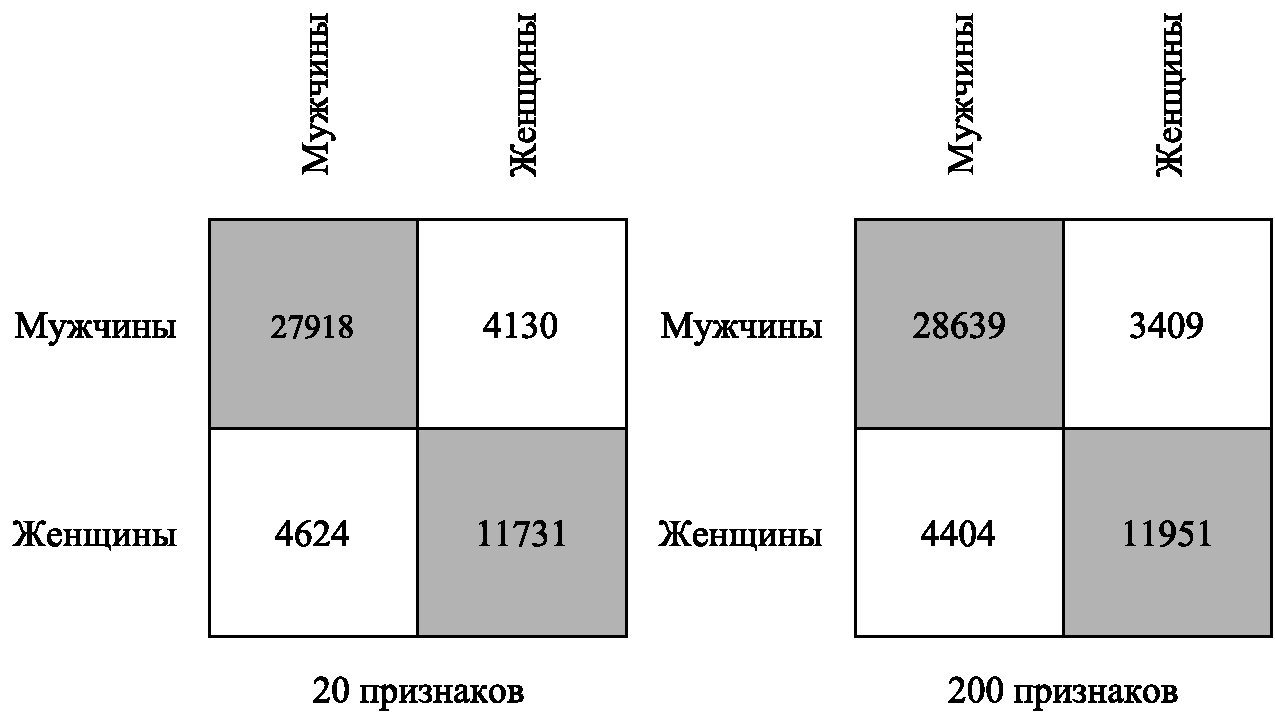
\includegraphics[scale=0.8]{figs/bow-we-confusion.pdf}
\end{figure}

В таблице~\ref{tab:order_we} приведены результаты
экспериментов с применением подходов вычисления матрицы
<<исполнитель-пользователь>> на основе порядка следования
исполнителей и word embedding. Для модели, позволяющей
достигнуть лучших результатов, на рисунке~\ref{fig:order_we_conf}
приведены матрицы ошибок.

\begin{table}[!h]
    \caption{Результаты эксперимента с применением подходов
             вычисления матрицы <<исполнитель-пользователь>>
             на основе порядка следования исполнителей 
             и word ebmedding}
    \label{tab:order_we}
\centering
\begin{tabular}{|c|c|c|}\hline
    \boldmath$f(a)$ & \textbf{Определение пола} & \textbf{Определение возраста} \\\hline
    \multicolumn{3}{|c|}{\textbf{20 признаков}} \\\hline
    $\frac{1}{\log(a + 1)}$ & 80,38\% & 2,98 \\\hline
    $\frac{1}{\sqrt{a}}$ & \textbf{81,55\%} & \textbf{2,90} \\\hline
    $\frac{1}{a^2}$ & 72,27\% & 4,64 \\\hline
    $\frac{1}{a}$ & 78,92\% & 3,75 \\\hline
    $51 - a$ & 77,90\% & 3,48 \\\hline
    $\log{51} - \log{a}$ & 78,11\% & 3,39 \\\hline
    $\sqrt{51} - \sqrt{a}$ & 78,15\% & 3,42 \\\hline
    \multicolumn{3}{|c|}{\textbf{200 признаков}} \\\hline
    $\frac{1}{\log(a + 1)}$ & 78,56\% & 3,15 \\\hline
    $\frac{1}{\sqrt{a}}$ & 80,32\% & \textbf{2,99} \\\hline
    $\frac{1}{a^2}$ & 74,77\% & 4,42 \\\hline
    $\frac{1}{a}$ & \textbf{80,89\%} & 3,35 \\\hline
    $51 - a$ & 77,82\% & 3,49 \\\hline
    $\log{51} - \log{a}$ & 78,18\% & 3,40 \\\hline
    $\sqrt{51} - \sqrt{a}$ & 78,11\% & 3,42 \\\hline
\end{tabular}
\end{table}

\begin{figure}[!h]
\caption{Матрицы ошибок для задачи определения пола с
         применением подходов вычисления матрицы 
         <<исполнитель-пользователь>> на основе порядка следования
         исполнителей и word embedding}
\label{fig:order_we_conf}
\centering
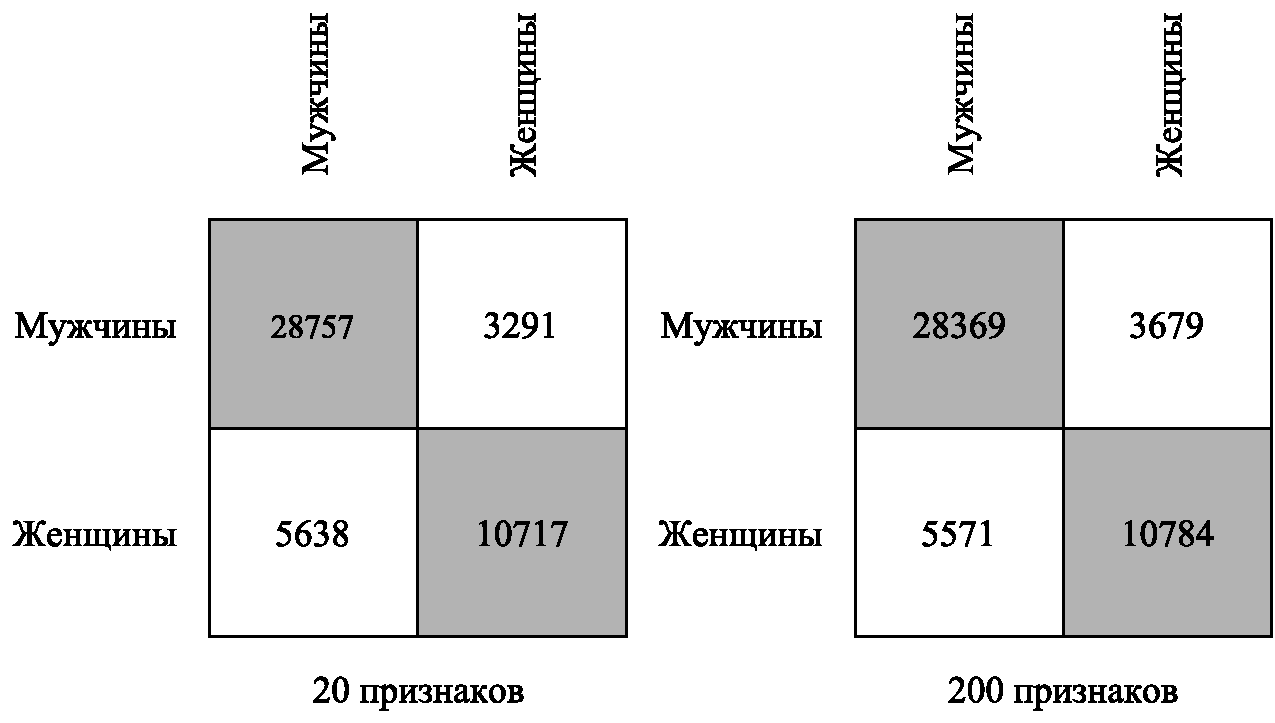
\includegraphics[scale=0.8]{figs/order-we-confusion.pdf}
\end{figure}

Как видно из результатов, подход к снижению размерности
матрицы <<исполнитель-пользователь>> на основе <<word embedding>>
позволяет достигать приемлемых результатов при малом числе признаков.
Напротив, подход, основанный на латентном семантическом анализе,
требует достаточно большого числа выбора признаков.

Также следует отметить, что подход на основе <<word embedding>>
позволяет решать задачу определения возраста пользователей сильно
лучше, чем подход на основе латентного семантического анализа.

Подход к вычислению матрицы <<исполнитель-пользователь>> на
основе порядка следования исполнителей в некоторых случаях
даёт улучшение результата, но наилучший результат получается
при применении формулы log-entropy в комбинации с word embedding.

Наконец, в таблице~\ref{tab:total_results} приведено сравнение
результатов, достигнутых в рамках настоящего исследования, и
результатов, полученных в работе~\cite{wu2014gender}.

\begin{table}[!h]
    \caption{}
    \label{tab:total_results}
\centering
\begin{tabular}{|c|c|c|}\hline
    \boldmath$f(a)$ & \textbf{Определение пола} & \textbf{Определение возраста} \\\hline
\end{tabular}
\end{table}

\chapterconclusion

Выводы выводы выводы
